%package list
\documentclass{article}
\usepackage[top=3cm, bottom=3cm, outer=3cm, inner=3cm]{geometry}
\usepackage{graphicx}
\usepackage{url}
%\usepackage{cite}
\usepackage{hyperref}
\usepackage{array}
\usepackage{multicol}
\newcolumntype{x}[1]{>{\centering\arraybackslash\hspace{0pt}}p{#1}}
\usepackage{natbib}
\usepackage{pdfpages}
\usepackage{multirow}
\usepackage{float}
\usepackage[normalem]{ulem}
\useunder{\uline}{\ul}{}


%%%%%%%%%%%%%%%%%%%%%%%%%%%%%%%%%%%%%%%%%%%%%%%%%%%%%%%%%%%%%%%%%%%%%%%%%%%%
%%%%%%%%%%%%%%%%%%%%%%%%%%%%%%%%%%%%%%%%%%%%%%%%%%%%%%%%%%%%%%%%%%%%%%%%%%%%
\newcommand{\csemail}{vmachacaa@unsa.edu.pe}
\newcommand{\csdocente}{Vicente Machaca Arceda}
\newcommand{\cscurso}{Algoritmos y Estructura de Datos}
\newcommand{\csuniversidad}{Universidad Nacional de San Agustín}
\newcommand{\csescuela}{Maestría en Ciencia de la Computación}
\newcommand{\cspracnr}{01}
\newcommand{\cstema}{--}
%%%%%%%%%%%%%%%%%%%%%%%%%%%%%%%%%%%%%%%%%%%%%%%%%%%%%%%%%%%%%%%%%%%%%%%%%%%%
%%%%%%%%%%%%%%%%%%%%%%%%%%%%%%%%%%%%%%%%%%%%%%%%%%%%%%%%%%%%%%%%%%%%%%%%%%%%


\usepackage[english,spanish]{babel}
\usepackage[utf8]{inputenc}
\AtBeginDocument{\selectlanguage{spanish}}
\renewcommand{\figurename}{Figura}
\renewcommand{\refname}{Referencias}
\renewcommand{\tablename}{Tabla} %esto no funciona cuando se usa babel
\AtBeginDocument{%
	\renewcommand\tablename{Tabla}
}

\usepackage{fancyhdr}
\pagestyle{fancy}
\fancyhf{}
\setlength{\headheight}{30pt}
\renewcommand{\headrulewidth}{1pt}
\renewcommand{\footrulewidth}{1pt}
\fancyhead[L]{\raisebox{-0.2\height}{
\includegraphics[width=3cm]{img/logo_unsa}}}
\fancyhead[C]{}
\fancyhead[R]{\fontsize{7}{7}\selectfont	\csuniversidad \\ \csescuela \\ \textbf{\cscurso} }
\fancyfoot[L]{MSc. Vicente Machaca}
\fancyfoot[C]{\cscurso}
\fancyfoot[R]{Página \thepage}

\begin{document}
	
	\vspace*{10px}
	
	\begin{center}	
		\fontsize{17}{17} \textbf{ Práctica \cspracnr}
	\end{center}
	%\centerline{\textbf{\underline{\Large Título: Informe de revisión del estado del arte}}}
	%\vspace*{0.5cm}
	

	\begin{table}[h]
		\begin{tabular}{|x{4.7cm}|x{4.8cm}|x{4.8cm}|}
			\hline 
			\textbf{DOCENTE} & \textbf{CARRERA}  & \textbf{CURSO}   \\
			\hline 
			\csdocente & \csescuela & \cscurso    \\
			\hline 
		\end{tabular}
	\end{table}	
	
	
	\begin{table}[h]
		\begin{tabular}{|x{4.7cm}|x{4.8cm}|x{4.8cm}|}
			\hline 
			\textbf{PRÁCTICA} & \textbf{TEMA}  & \textbf{DURACIÓN}   \\
			\hline 
			\cspracnr & Algoritmos de Ordenamiento & 3 horas   \\
			\hline 
		\end{tabular}
	\end{table}
	
	
	\section{Datos de los estudiantes}
	\begin{itemize}
		\item Grupo: V
		\item Integrantes: 
		\begin{itemize}
			\item Angel Yvan Choquehuanca Peraltilla
			\item Estefany Pilar Huaman Colque
            \item Eduardo Diaz Huayhuas
            \item Gustavo Raul Manrique Fernandez
		\end{itemize}		
	\end{itemize}
	
	
 
	



	
	


	
	%\clearpage
	%\bibliographystyle{apalike}
	%\bibliographystyle{IEEEtranN}
	%\bibliography{bibliography}
		

    \section{Introducción}
    Se considera un algoritmo de ordenamiento a un conjunto de ordenes que permite que: A un vector o conjunto de datos se le aplique acciones de reordenamiento. Este algoritmo puede ser de diferente tipo de secuencias con el mismo fin. 

    Desde la aparición del primer algoritmo (BubbleSort en 1956), la formulación de algoritmos viene siendo un caso de estudio por cientificos afines a la materia.

    Con el pasar de los años se ha clasificado los algoritmos de acuerdo al metodo de ordenamiento.
    En este informe se aborda el analisis de tiempo en ejecución de diferentes algoritmos en los lenguajes Python, C++ y Go.
    
    \section{Datos del Equipo}
    Se utilizó un equipo en la nube proporcionado por Replit (www.replit.com) con las siguientes caracteristicas:

    \begin{itemize}
        \item 0.5vCPU con Ubuntu 21.04-KVM
        \item 1 GB de Memoria RAM
        \item 1 TB de disco SSD
    \end{itemize}

    \section{Metodologia y Desarrollo}
    Para realizar las experiencias tomaron en cuenta los siguientes aspectos:
    
    \begin{enumerate}
        \item Se preparó los datos a partir de un generador de valores en Python mediante la libreria \textit{random}. Estos valores son usados para los 3 lenguajes en su ejecución.
        \item Se subieron los archivos en la maquina virtual proporcionado por Replit.
        \item Se preparó el entorno de trabajo separado por carpetas e instalando los compiladores adecuados.
        \item Se utilizó el comando \textbf{time} de Linux para calcular el tiempo de ejecución real y del sistema.
        \item Se hace 5 pruebas por cada ejecución y se grabaron los resultados en una tupla en \textit{Google Colab}.
        \item Se hace uso de la libreria \textbf{MatPlotLib} de Python para la realización de los calculos estadisticos y graficos.
    \end{enumerate}

\section{Resultados}
Para MergeSort 
    \begin{figure}[h!]
        \centering
        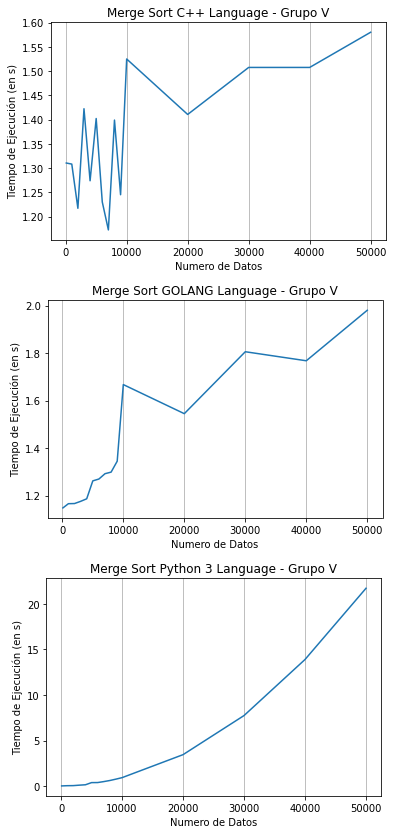
\includegraphics[scale=0.4]{img/finalmerg.png}
        \caption{Algoritmo MergeSort}
        \label{fig:my_label}
    \end{figure}

\begin{table}[t]
\begin{center}
\begin{tabular}{| c | c | c | c | c | c | c |}
\hline
\multicolumn{7}{ |c| }{Algoritmo MergeSort - Promedios y Desviacion Estandar} \\ \hline
Datos & C++ (s) & Go (s) & Py (s) &  DE C++ & DE Go & DE Py\\ \hline
100 & 1.3104 & 1.1484 & 0.0352 & 0.11226 & 0.07171 & 0.00444 \\
1000 & 1.3082 & 1.1662 & 0.0596 & 0.12914 & 0.03769 & 0.00417 \\
2000 & 1.217 & 1.1667 & 0.068 & 0.11981 & 0.03166 & 0.00572 \\
3000 & 1.4224 & 1.176 & 0.118 & 0.07406 & 0.03871 &  0.00993 \\
4000 & 1.2738 & 1.1868 & 0.1612 & 0.074405 & 0.017982 & 0.00495 \\
5000 & 1.4022 & 1.2622 & 0.3974 &  0.07954 & 0.01495 & 0.04623 \\
6000 & 1.23 & 1.27 & 0.4034 & 0.073759 & 0.02530 &  0.01382 \\
7000 & 1.1724 & 1.2924 & 0.5084 & 0.10504 & 0.01942 & 0.01861 \\
8000 & 1.3989 & 1.299 & 0.6282 & 0.10770 & 0.02265 & 0.03787 \\
9000 & 1.2449 & 1.345 & 0.7786 & 0.08257 & 0.02566 & 0.02032 \\
10000 & 1.525 & 1.6674 & 0.94 &  0.02795 & 0.06302 & 0.048985 \\
20000 & 1.4105 & 1.545 & 3.4601 & 0.10274 & 0.12826 &  0.1004 \\
30000 & 1.5076 & 1.8056 & 7.7452 &  0.07759 & 0.05421 & 0.176682 \\
40000 & 1.5076 & 1.7676 & 13.8876 & 0.07759 &  0.04846 & 0.66075 \\
50000 & 1.5802 & 1.9802 & 21.6906  & 0.03328  &  0.08478 & 0.71114 \\ \hline
\end{tabular}
\caption{Tiempo de Ejecución, en segundos}
\label{tab:coches}
\end{center}
\end{table}



\section{Conclusiones}
En MergeSort 
    \begin{itemize}
        \item El enguaje C++ utiliza menos tiempo en ejecutar este algoritmo (entre 1 a 2 segundos). Y que, puede ejecutar cargas de millones de datos en tiempos menores. 
        \item El lenguaje Go utiliza similar tiempo con el C++, pero a su vez tiende a aumentar linealmente su tiempo de ejecución. Ambos lenguajes anteriormente mencionados son derivados del C.
        \item Para el lenguaje Python, este muestra un aumento del tiempo exponencial. La razon es sencilla: y es que este lenguaje es interpretado, o sea, mientras compila el programa, ejecuta las funciones. Y por tal para algunos procesamientos de millones de datos puede que no sea tan efectivo.
        
    \end{itemize}
\end{document}
